\documentclass{article}
\usepackage{tikz}
\usetikzlibrary{arrows.meta,positioning,calc,shapes.geometric}
\pagestyle{empty}
\begin{document}
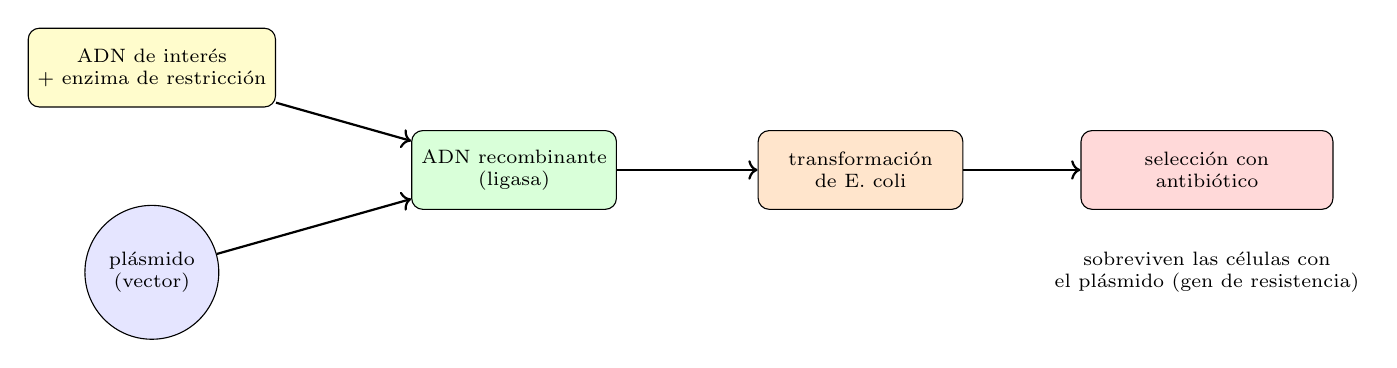
\begin{tikzpicture}
\tikzset{every node/.append style={align=center}}

\node[draw, rounded corners, fill=yellow!20, minimum width=2.6cm, minimum height=1.0cm, align=center, font=\scriptsize] (g) at (0,3.0) {ADN de interés\\ + enzima de restricción};
\node[draw, circle, fill=blue!10, minimum size=1.7cm, align=center, font=\scriptsize] (v) at (0,0.4) {plásmido\\ (vector)};
\node[draw, rounded corners, fill=green!15, minimum width=2.6cm, minimum height=1.0cm, align=center, font=\scriptsize] (r) at (4.6,1.7) {ADN recombinante\\ (ligasa)};
\node[draw, rounded corners, fill=orange!20, minimum width=2.6cm, minimum height=1.0cm, align=center, font=\scriptsize] (t) at (9.0,1.7) {transformación\\ de E. coli};
\node[draw, rounded corners, fill=red!15, minimum width=3.2cm, minimum height=1.0cm, align=center, font=\scriptsize] (s) at (13.4,1.7) {selección con\\ antibiótico};
\draw[->, thick] (g) -- (r); \draw[->, thick] (v) -- (r); \draw[->, thick] (r) -- (t); \draw[->, thick] (t) -- (s);
\node[font=\scriptsize, align=center] at (13.4,0.4) {sobreviven las células con\\ el plásmido (gen de resistencia)};

\end{tikzpicture}
\end{document}
